\documentclass{article}
\usepackage{titling}
\usepackage{lipsum}
\usepackage{amsmath}
\usepackage{listings}
\usepackage{graphicx}
\usepackage{subcaption}
\usepackage{pgfplots}
\usepackage{float}
\usepackage[margin=1in]{geometry}
\usepgfplotslibrary{statistics}



\begin{document}
\noindent
\begin{minipage}[t]{0.6\textwidth}
    \begin{flushleft}
        \LARGE\textbf{CSCI 347 - Project 3 Report} \\
        \vspace{6pt} % add 6pt of vertical space
        \hrule width 10cm
        \vspace{12pt}
        \large\textbf{Preston Duffield} \\
        \large Western Washington University \\
        \today
        \vspace{24pt}
    \end{flushleft}
\end{minipage}

\section*{Edge Detector}
Edge Detector is an edge detection program that uses a
Laplacian filter to highlight the edges in a set of images.
The images are specified as command line arguments and the project
is designed to process multiple images concurrently using threads.
The goal of the project is to concurrently apply the laplacian
filter to multiple images, improving the execution time
compared to sequential execution. \\
\begin{flushleft}
  The program contains several functions, structs,
  and a global variable, all of which work together to process the images:
\end{flushleft}
\begin{enumerate}
  \item \texttt{PPMPixel} Struct: This struct represents a pixel in an image, with the RGB values of the pixel.
  \item \texttt{parameter} Struct: This struct holds the information each thread needs to perform its task.
  \item \texttt{file\_name\_args} Struct: This struct is used to hold the input and output filenames for each image.
  \item \texttt{total\_elapsed\_time} Global Variable: This is a double value that tracks the total time taken by all threads to process all input images.
  \item \texttt{compute\_laplacian\_threadfn}: This is the thread function. It applies the Laplacian filter to a section of the image.
  \item \texttt{apply\_filters}: This function uses threads to apply the Laplacian filter to an image and measures the time taken.
  \item \texttt{write\_image}: This function saves a processed image to a file.
  \item \texttt{read\_image}: This function reads an image file and returns a PPMPixel pointer to the pixel data.
  \item \texttt{manage\_image\_file}: This is another thread function. It manages the entire process of reading an image file, processing the image, and writing the result to a file.
  \item \texttt{main}: This is the entry point of the program. It checks command line arguments, creates threads to process each image file, and prints the total elapsed time.
\end{enumerate}

\subsection*{Shell Script}
Edge detector can be run from a shell script.
The script, \texttt{run\_program.sh}, accepts a directory as a command line argument.
It then collects all of the \texttt{.ppm} files and passes them as input into the edge detection program.

\clearpage
\section*{Concurrency}
Concurrency in this program is achieved through the use of POSIX threads (pthreads).
For each image file passed as a command line argument,
a new thread is created in the main function.
Each of these threads runs the \texttt{manage\_image\_file} function,
which manages the processing of one image.\\

Within the \texttt{manage\_image\_file} function,
the \texttt{apply\_filters} function is called,
which further divides the work among a specified number of threads
(defined by the \texttt{LAPLACIAN\_THREADS} macro).
Each of these threads runs the \texttt{compute\_laplacian\_threadfn} function,
which applies the Laplacian filter to a section of the image.\\

In terms of handling possible race conditions,
the main area where this could occur is when updating the \texttt{total\_elapsed\_time}
global variable. However, as each image file is processed
by a separate thread and the time taken to process each image is
added to \texttt{total\_elapsed\_time} in a single operation, there's no risk of
race conditions here as the operation is atomic.
Furthermore, as the processed images are written to separate files,
there is no risk of a race condition when writing the output.\\

\section*{Experiment}
The following experiment was run on a 2.2 GHz 6-Core Intel Core i7 processor.
A Python program\footnote{See Appendix} was written to run \texttt{run\_program.sh} 10 times and record the results to a .csv file.
Each time the program was run on 40 images of various sizes.
10 replicants (runs) were performed for each test and the times where noted.
Using the same photos, run amounts, and processor, we can isolate our variable, which is the amount of threads that \texttt{edge\_detector.c} opens.
The experiement was run with \texttt{LAPLACIAN\_THREADS}, the value which defines the number of threads that work on a single image, set to values 1 through 16.
The experiment was run 16 times, with 10 replicants each, for a total of 160 data points.

\subsection*{Experiemental Design Summary}
\begin{flushleft}
  \textbf{Variables:} The value of \texttt{LAPLACIAN\_THREADS}, tested from 1 to 16. \\
\end{flushleft}

\begin{flushleft}
  \textbf{Response:} The combined time in seconds needed for each thread to complete its task. \\
\end{flushleft}

\begin{flushleft}
  \textbf{Replicants:} 10 replicants for each level of \texttt{LAPLACIAN\_THREADS}, for a total of 160 data points. \\
\end{flushleft}

\begin{flushleft}
  \textbf{Constants:}
  \begin{itemize}
    \item 40 images were processed in each run.
    \item each test was run on the same processor.
  \end{itemize}
\end{flushleft}

\clearpage
\section*{Results}
\begin{figure}[h]
  \centering
  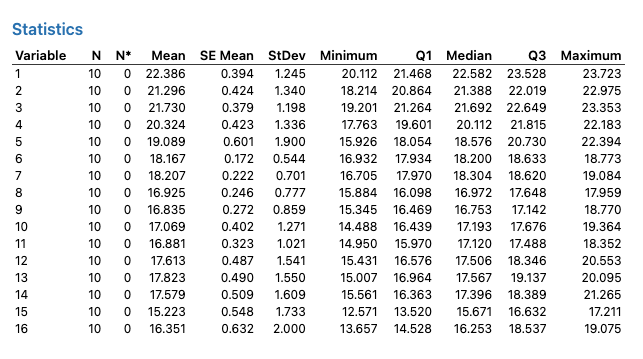
\includegraphics[width=1\textwidth]{./images/3.png}
  \caption{Descriptive statistics of the data.}
  \label{fig:3_b_2}
\end{figure}

The descriptive statistics of the data show that the means are grouped around the values of around 16 to 23 seconds.
Note that "N" is the amount of replicants, and "Variable" is the amount of laplacian threads.

\begin{figure}[h]
  \centering
  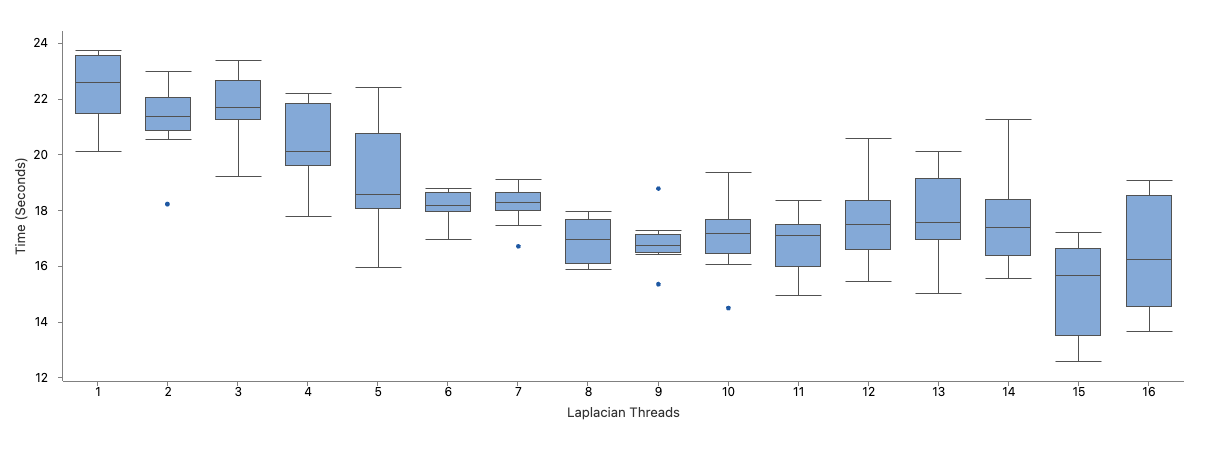
\includegraphics[width=1\textwidth]{./images/2.png}
  \caption{Boxplot of the data.}
  \label{fig:3_b_2}
\end{figure}
The boxplot shows the spread in the data from each test performed. Note that from around threads 6 to 9, the data is less spread out, ie has a smaller standard deviation than other values.
The dots indicate outliers, these are single data points that lie outside the interquartile range of the data for a single test.

\clearpage
\begin{figure}[h]
  \centering
  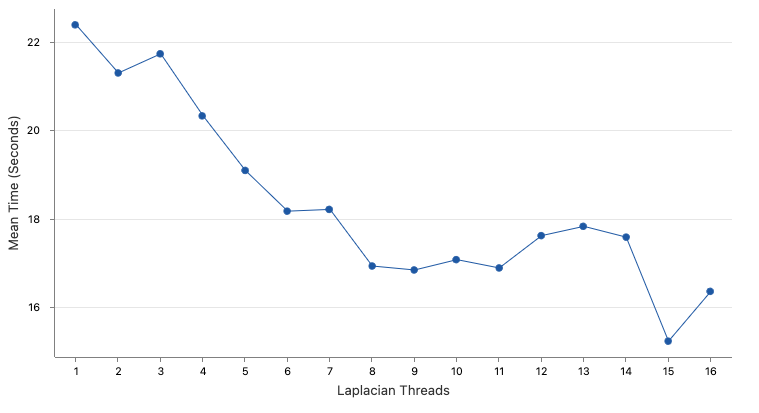
\includegraphics[width=1\textwidth]{./images/1.png}
  \caption{Line plot of means.}
  \label{fig:3_b_2}
\end{figure}
This lineplot shows the mean for each replicant of each test connected by a line.
That is, each dot represents the average of all 10 invocations of
\texttt{edge\_detector} at a given thread amount, from 1 to 16.

\section*{Implications of Results}
From the boxplot we note that the spread of the data,
ie, the standard deviation is lower for the thread counts 6,7,8,9.
This could be related to the fact that the processor the experiment was
ran on had 6 total cores.
However, more experiments on systems with different core counts
would be needed to verify this.
Thus we cannot say with certainty that this change in spread
is anything but a statistical anomally,
but it is an interesting result nonetheless. \\

The lineplot seems to show the mean time in seconds decreasing
as the laplacian threads increase. This increase is most significant
from 1 to 6 threads, however, after that it appears to reach an
asymptote at around 17 seconds. This seems to indicate that increasing
the amount of threads decreases the mean time in seconds up to a certain amount.
\section*{Conclusion}
The results of the experiment provide some interesting insights into the
concurrent processing of images using the Edge Detector program. \\

In the given setting, the number of Laplacian threads has a significant
impact on the overall processing time, particularly when the number of
threads ranges from 1 to 6. The mean processing time reduces significantly
within this range, which corroborates the basic principle of concurrency
- that dividing the work among multiple threads can expedite the execution time. \\

However, the effects of concurrency are not linear, and the data starts
to plateau after around 6 threads, reaching an asymptote at approximately
17 seconds. This suggests that there is a limit to the performance
improvement that can be achieved through increasing the number of threads.
Beyond a certain point, the overhead of creating and managing more threads
may start to negate the performance benefits of concurrency. \\

The decrease in data spread for thread counts between 6 and 9 is also
noteworthy. This result aligns with the 6-core architecture of the test
processor, and it may imply an optimal thread count per core. However,
this hypothesis requires further testing on processors with different core counts to confirm. \\

Overall, the Edge Detector program successfully leverages the power
of concurrency to enhance its performance. The optimal number of threads
to achieve the fastest processing time appears to be dependent on the
processor architecture, specifically the number of cores. Therefore,
to optimize the performance of similar concurrent applications,
developers should take into account the characteristics of the target
hardware, including the number of cores and the cost of thread management.
Future studies could investigate how other factors, such as the size and
complexity of the images, may also impact the performance of concurrent
image processing applications. \\

\clearpage
\appendix
\section*{Appendix}
\subsection*{Python Program}
\begin{lstlisting}[language=Python, 
  basicstyle=\ttfamily\small, 
  numbers=none, 
  frame=single, 
  caption={A Python program that runs \texttt{run\_program.sh} 10 times and records the results to a csv file.},
  label=code:min_penalty_path,
  escapeinside={(*}{*)}]
  import sys
  import subprocess
  import csv
  import os
  import re
  
  def run_edge_detector(times, image_folder):
      # Check if the given folder exists
      if not os.path.isdir(image_folder):
          print("Image folder not found")
          return
  
      # Check if run_program.sh exists
      if not os.path.isfile("./run_program.sh"):
          print("run_program.sh not found")
          return
  
      # Prepare the csv file
      with open('output.csv', 'w', newline='') as file:
          writer = csv.writer(file)
          writer.writerow(["Seconds"])
  
          # Loop to run the edge detector for the given number of times
          for i in range(times):
              try:
                  print("Run: ", i)
                  # Run the shell script with the image folder as an argument
                  process = subprocess.Popen(
                    ['./run_program.sh', image_folder],
                    stdout=subprocess.PIPE, stderr=subprocess.PIPE)
                  stdout, stderr = process.communicate()
                  # Check for errors in the shell script
                  if process.returncode != 0:
                      print(f"Error in run_program.sh: {stderr.decode('utf-8')}")
                      continue
                  # Extract the time from the output using regular expressions
                  match = re.search(r"Total elapsed time: (\d+\.\d+) s"\,
                    stdout.decode('utf-8'))
                  if match:
                      writer.writerow([match.group(1)])
                  else:
                      print("Could not extract time from run_program.sh output")
  
              except Exception as e:
                  print(f"Unexpected error: {e}")
  
  if __name__ == "__main__":
      # Check if the correct number of arguments was given
      if len(sys.argv) != 3:
          print("Usage: python3 run_edge_detector.py <times> <image_folder>")
          sys.exit(1)
      # Run the edge detector
      run_edge_detector(int(sys.argv[1]), sys.argv[2])
  
\end{lstlisting} 

\end{document}
